\chapter{Consenso}

Aplicações em sistemas distribuídos são tipicamente complicadas para se construir, por causa desse fator de consenso entre os participantes. Existe uma grande motivação em garantir consenso entre os participantes e, a razão disso é a necessidade de fazer com que o sistema distribuído evolua igualmente por todos os participantes. Segundo \cite{lamport2001paxos} os algoritmos de consenso precisam garantir 3 propriedades de segurança:

\begin{itemize}
\item Não trivialidade: Um valor aprendido se e somente se tiver sido proposto, e aceito pela maioria dos participantes.

\item Estabilidade: A cada rodada de aprendizagem, qualquer processo participantes pode aprender no máximo um valor. Um valor aprendido não pode ser alterado posteriormente, pois um valor aprendido será executado na aplicação.

\item Consistência: A cada rodada de aprendizagem, dois processos diferentes não podem aprender valores diferentes. 
\end{itemize}

\section{Replicação Máquinas de Estados}

O uso de Replicação por Máquina de Estados (RMS) foi proposto por \textcite{schneider1990} e, é comumente discutida na literatura o uso de RMS baseada em \textit{logs} \cite{lamport2001paxos}. Uma vantagem de usarmos máquina de estado é a promoção de tolerância a falhas e, o aumento da disponibilidade do sistema \cite{lamport1978implementation, schneider1990}. Por enquanto estamos considerando o módulo de consenso como uma caixa preta, que é utiliza pelo mecanismo de máquina de estados (a figura \ref{fig:rms} explica melhor esse cenário). De maneira geral, para a replicação por máquinas de estados funciona da seguinte forma: Configuramos um \textit{cluster} com várias máquinas replicando um mesmo serviço (\textit{i.e.} Banco de dados), e a medida que os clientes fazem suas requisições, a máquina de estados age como um replicador de \textit{logs}. Uma pré-condição para que todas as réplicas de máquina de estado se comportem de forma idêntica é executar as mesmas entradas de comando na mesma ordem. Os \textit{logs} aqui são as instruções que vão alterar dados da aplicação que o \textit{cluster} está servindo \cite[p.~216]{PauloVerissimoLuisRodrigues}.

Implementar replicação por máquina de estados fornece tolerância a falhas. Também fornece escalabilidade, pois os clientes podem ler dados de qualquer servidor disponível.

Para manter o conteúdo replicado, temos duas opções de design \cite{wtf2018}:

\begin{itemize}
\item Apenas 1 mestre fixo que recebe todas as solicitações, e repassa essas solicitações para os demais participantes do sistema.
\item Qualquer réplica pode se tornar um mestre eventualmente, através de um algoritmo de eleição.
\end{itemize}

Existem duas primitivas envolvidas em RME:

\begin{enumerate}
\item \textit{invoke(operation)}: essa primitiva é executada pelos clientes para chamar operações no serviço que implementa RME.
\item \textit{execute(operation)}: essa primitiva é executada pelos servidores replicados, sempre que uma operação deve ser executada pelo serviço de RME.
\end{enumerate}

Além disso existem algumas propriedades para tornar o RME determinístico.

\begin{itemize}
\item Estado inicial: todas as réplicas corretas devem inciar a partir de um mesmo estado.
\item Determinismo: todas as réplicas corretas, que executam uma mesma operação sobre um mesmo estado, realizam a mesma mudança em seus estados e produzem a mesma resposta.
\item Coordenação: todas as réplicas corretas executam a mesma sequência de operações.
\end{itemize}

\subsection{Replicação Ativa}

Difusão atômica é uma primitiva que tem influência quando se implementa replicação ativa \cite{lamport1978implementation, schneider1990}. A replicação ativa é uma técnica intuitiva que pode ser aplicada a máquinas de estado. Consiste em ter várias réplicas da mesma máquina de estado executadas por diferentes processos. Para garantir que o estado dessas réplicas seja mantido consistente, um protocolo de ordenação total deve ser usado para difundir os comandos da máquina de estado, no caso do \cite{PauloVerissimoLuisRodrigues}.

Essa máquina de estados deve estar presente em cada réplica, e compartilhar um \textit{log} em comum e, a ideia é executar comandos do \textit{log}, igualmente em cada réplica, como é possível ver na figura \ref{fig:rms}. Os comandos do \textit{logs} são comandos que foram autorizados por um algoritmo de consenso.

\begin{figure}[htb!]
\centering
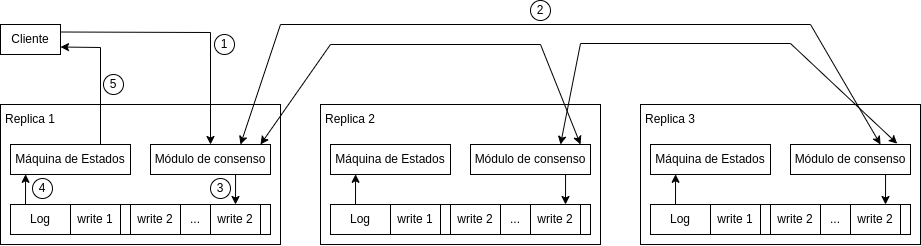
\includegraphics[width=1\linewidth]{figures/rms.drawio.png}
\caption{Fonte: Adaptado de \textcite[p.~233]{journals/dbsk/SkrzypzcakS20}}
\label{fig:rms}
\end{figure}

A imagem \ref{fig:rms} mostra que em um sistema distribuído essa máquina de estados deve ser replicada, ou seja, todos os servidores deste sistema distribuído deverão executar a mesma máquina de estados. As marcações numeradas na figura são respectivamente:

\begin{enumerate}
\item Envia um comando qualquer para a Máquina de Estados Replicada.
\item Entre em consenso sobre o comando.
\item Concatena o novo comando.
\item Aplica o comando que está na fila para ser executado, e que está no \textit{log}.
\item Responde ao cliente.
\end{enumerate}

Mas o que realmente é essa máquina de estados replicada? Cada nó, de um sistema distribuído, Pode ser pensado como uma máquina de estados determinística. O intuito é prover tolerância a falhas, executando o mesmo registro de comandos, após cada ponto de salvamento. Idealmente essa é a ideia básica, porém na realidade existem  complicações, essas complicações motivam a pesquisa e desenvolvimento desse trabalho acadêmico. A imagem a seguir exemplifica, de maneira abstrata, como seria a replicação máquina de estados paralela. O desafio aqui é replicar o registro de comandos, igualmente, para todas as máquinas do sistema. Depois da replicação feita é necessário impor uma sincronização para que eles executem os comandos e a aplicação \textit{stateful} transite de estado, gerando um novo estado, porém são várias aplicações replicadas e iguais ao final do processo.

\subsection{Procolos de Consenso}

O problema de Consenso surgiu da necessidade de múltiplos computadores que compartilham o estado do sistema, chegarem à um acordo sobre determinado valor. Ou seja, para atingirmos harmonia entre os participantes de um sistema distribuído de computadores precisamos de um algoritmo capaz de estabelecer um inquérito entre as máquinas. Veja que até o momento não precisamos mencionar se existe um tipo de aplicação específica, pois esse consenso é algo anterior a isso e, que deve estabelecer um acordo sobre algum comando antes desse comando ser executado por uma determinada aplicação.

A seguir veremos duas tecnologias, bastante conhecidos, na literatura e, que implementam consenso, tipicamente ambos tem a intenção de oferecer uma evolução gradual e baseada em máquina de estados, da replicação dos \textit{logs} internos que contêm comandos que irão alterar o estado interno de uma aplicação.

\subsubsection{Paxos}

O algoritmo Paxos foi desenvolvido por \cite{lamport2001paxos}. É um algoritmo usado para obter consenso sobre um determinado valor. Geralmente se implementa Paxos entre um conjunto distribuído de computadores trocando mensagens de forma assíncrona. Por exemplo, um cliente propõem um valor ao sistema, e o protocolo Paxos é invocado para propor o valor, quando a maioria dos participantes que executam o Paxos concordarem sobre o valor proposto, então o valor proposto deve ser considerado como aprendido e será absorvido pelo sistema. A proposta parte de algum dos participantes do sistema que está atuando como líder no momento da proposição. Existem 3 papéis no algoritmo Paxos:

\begin{itemize}
\item O proponente (\textit{proposer})
\item Os aceitadores (\textit{acceptors})
\item O aprendiz (\textit{learner})
\end{itemize}

O algoritmo Paxos tem basicamente 2 fases, a seguir vamos descrever as fases, brevemente:

\textbf{Primeira fase: Preparação}

\begin{itemize}

\item O proponente, ou remetente, irá propor um valor enviando mensagens para os destinatários através da difusão.

\item Os aceitadores, ou destinatários, irão avaliar a proposta de valor, e emitir suas respostas, sinalizando que reconheceram a mensagem $m$. Os aceitadores só respondem a propostas com número de sequência único e maior do que o anterior.
\end{itemize}

\textbf{Segunda fase: Aceitação}

\begin{itemize}
\item O aprendiz aprende se os destinatários chegaram a um consenso em uma rodada específica do algoritmo. A quantidade de destinatários precisa ser pelo menos metade do conjunto de servidores do sistema.
\end{itemize}

\subsubsection{Raft}

Raft foi desenvolvido por \cite{raft}. Trata-se de um algoritmo de consensus que garante que as replicas cheguem à um mesmo acordo. Os autores procuraram ser bastante didáticos ao construir esse algoritmo. Esse algoritmo espera que exista um sistema distribuído replicado por máquinas de estados determinísticas. É um algoritmo assimétrico, no sentido de que, os candidatos elegem um líder. Cada candidato é, no caso, um nó do sistema distribuído. Existem três estados que um candidato Pode alcançar, são eles: \textit{líder}, candidato, seguidor. A figura a seguir, Poderá esclarecer bastante como que um nó do sistema Pode alternar de estados, e quando ele Pode. A ideia básica é alternância de liderança, ou eleição democrática.

\begin{figure}[h] % ’ht’ tells LaTeX to place the figure ’here’ or at the top of the page
\centering
\begin{tikzpicture}
\tikzset{->, >=stealth, node distance=5cm, every state/.style={thick, fill=gray!10}, initial text=Início}
\node[state, accepting, initial] (q1) {$Seguidor$};
\node[state, accepting, right of=q1] (q2) {$Candidato$};
\node[state, accepting, right of=q2] (q3) {$\text{Líder}$};
\draw
(q2) edge[loop above] node{{\tiny acabou o tempo, nova eleição}} (q2)
(q1) edge[bend left, above] node{{\tiny acabou o tempo, começa eleição}} (q2)
(q2) edge[bend left, above] node{{\tiny recebe votos da maioria}} (q3)
(q2) edge[bend left, below] node{{\tiny descobre novo \text{líder}}} (q1)
(q3) edge[bend left, below] node{{\tiny descobre servidor com prioridade na liderança}} (q1);
\end{tikzpicture}
\caption{Fonte própria. Máquina de estados representando as fases de um nó servidor, dentro do esquema Raft}
\end{figure}

Mas o que acontece em cada um desses estados?

\begin{itemize}
\item Os seguidores apenas ficam escutando o líder, e se depois de um tempo eles não escutaram nada do líder, eles viram candidatos.
\item Os autores do Raft, desenvolveram um mecanismo para decidir sobre informações obsoletas. Esse mecanismo se chama \textbf{termo}.
\item A ordem de prioridade dos termos aumentam de acordo com qual termo é mais recente. Ou seja, termos mais recentes são mais importantes. Existe então alguma noção de tempo inserida no algoritmo Raft.
\item É necessário haver um número específico de servidores operacionais, para Poder manter o mecanismo de eleição democrático. Pois se um servidor falhar, algum outro candidato irá eventualmente entrar em \textit{timeout}, e consequentemente irá tentar ganhar a eleição.
\item O seguidor vota por qualquer um que chegar primeiro, \textit{First Come First Served}.
\item O líder entrar em comando do \textit{Cluster}, e é responsabilidade dele de replicar o \textit{log} em todas as réplicas.
\item A regra chamada vivacidade (do Inglês \textit{liveness}). Se trata da escolha do tempo de espera até o \textit{timeout} de um nó servidor. A escolha do tempo até \textit{timeout} é feito de maneira aleatória, não compromete a \textit{eleição}, em até pelo menos 1 termo de folga.
\item A regra chamada \textbf{segurança} garante apenas 1 líder por termo.
\end{itemize}

\subsubsection{Comparação entre Raft e Paxos}

Em termos de provas formais, ambos buscam formalizar em provas matemáticas e premissas imutáveis, basicamente 4 regras formais dão embasamento formal. As regras formais são propriedades para atingir consenso assíncrono entre as partes envolvidas. A partir de estudos posteriores, os autores \textcite{MOSTEFAOUI_RAYNAL} esmiuçaram 4 regras formais e, que hoje estão elucidadas nas premissas a seguir:

% The Consensus Problem
% In the Consensus problem, every correct process Pi proposes a value v\ and all
% correct processes have to decide on the same value v, that has to be one of the
% proposed values. More precisely, the Consensus problem is defined by three safety
% properties (Validity, Integrity and Uniform Agreement) and a Termination Property
% [4,10]:
% [4] Chandra T. and Toueg S., Unreliable Failure Detectors for Reliable Distributed Systems. Journal of the ACM, 43(2):225-267, March 1996
% [10] Fischer M.J., Lynch N. and Paterson M.S., Impossibility of Distributed Consensus with One Faulty Process. Journal of the ACM, 32(2):374-382, April 1985
% • Validity: If a process decides v, then v was proposed by some process.
% • Integrity: A process decides at most once.
% • Uniform Agreement: No two processes decide differently.
% • Termination: Every correct process eventually decides on some value.

\begin{enumerate}
\item Validade: apenas os valores propostos podem ser decididos. Se um processo decidir sobre um valor, v, então algum processo precisa ter proposto v.
\item Acordo uniforme: dois processos corretos (aqueles que não falham), não podem decidir sobre valores diferentes.
\item Integridade: cada processo pode decidir 1 valor pelo menos 1 vez.
\item Termo: todos os processos vão, eventualmente, decidir sobre um resultado.
\end{enumerate}

% O Kubernetes, por padrão, não permite que StatefulSets obedeçam a terceira regra, Integridade. Apenas o nó mestre pode escrever na aplicação stateful, e se o nó mestre falhar outro nó deve ser eleito mestre, do contrário o cluster não irá mudar.

Em termos de sistemas distribuídos, ambos servem casos de uso semelhantes, por exemplo: ``Como múltiplas réplicas podem chegar à uma conclusão sobre um único comando?''. Paxos generalmente sacrifica disponibilidade \cite{cason2017role}, e o Raft opera as custas de disponibilidade. Quando nos deparados com particionamento de redes, Paxos vai continuar disponível, mas o \textit{cluster} Raft pode ficar parcialmente indisponível. Raft, e Paxos, são algoritmos de consenso que confiam na maioria do \textit{cluster}, em constante comunicação, para evoluir de estado. Em termos de didática, Raft tem um propósito de ser fácil de se compreender, enquanto Paxos não tem essa premissa. Ambos Paxos e Raft vão continuar operando enquanto o cluster enfrenta falhas em seus nós.